\begin{enumerate}[label=\alph*)]
    \item
        不是凸集, 理由如下:

        \begin{figure}[ht]
            \centering
            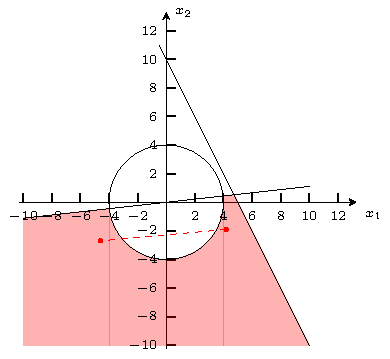
\includegraphics[scale=1.2]{figures/2a.pdf}
            \caption{}
            \label{figure:2a}
        \end{figure}
        如\cref{figure:2a}, 取图中两点连成线段, 该线段不在$S$内, 因此$S$不是凸集.
    \item
        是凸集, 理由如下:

        $\forall s_1=(x_1,y_1),s_2=(x_2,y_2)\in S$, 要证$S$是凸集, 即证$\forall\lambda\in[0,1]$, s.t.
        \begin{equation*}
            \lambda s_1+(1-\lambda)s_2
            =(x,y)
            =(\lambda x_1+(1-\lambda)y_1, \lambda x_2+(1-\lambda)y_2)
            \in S.
        \end{equation*}
        因为
        \begin{equation*}
            x + y
            =\lambda(x_1+y_1)+(1-\lambda)(x_2+y_2)
            \leq6,
        \end{equation*}
        \begin{equation*}
            -2x + 3y
            =\lambda(-2x_1+3y_1)+(1-\lambda)(-2x_2+3y_2)
            \geq2,
        \end{equation*}
        \begin{equation*}
            4x - y
            =\lambda(4x_1-y_1)+(1-\lambda)(4x_2-y_2)
            \leq12,
        \end{equation*}
        则$(x,y)\in S$, 因此$S$是凸集.

    \item
        是凸集, 理由如下:

        $\forall s_1=(x_1,y_1),s_2=(x_2,y_2)\in S$, 要证$S$是凸集, 即证$\forall\lambda\in[0,1]$, s.t.
        \begin{equation*}
            \lambda s_1+(1-\lambda)s_2
            =(x,y)
            =(\lambda x_1+(1-\lambda)y_1, \lambda x_2+(1-\lambda)y_2)
            \in S.
        \end{equation*}
        易证$x+y\geq3, x\geq1$, 因此只需证明$-(x-1)^2+y\geq1$即可.

        令$f(x)=-(x-1)^2$, 则$f''(x)=-2\leq0$, 因此函数$f(x)$是凹函数, 即
        \begin{equation*}
            -(x-1)^2\geq -\lambda(x_1-1)^2-(1-\lambda)(x_2-1)^2.
        \end{equation*}
        又因为$y=\lambda x_2+(1-\lambda)y_2$, 所以
        \begin{equation*}
            -(x-1)^2+y\geq \lambda[-(x_1-1)^2+y_1]+(1-\lambda)[-(x_2-1)^2+y_2]\geq1.
        \end{equation*}
        因此$S$是凸集.

    \item
        不是凸集, 理由如下:

        \begin{figure}[ht]
            \centering
            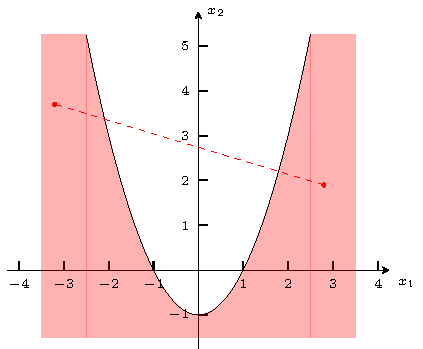
\includegraphics[scale=1.2]{figures/2d.pdf}
            \caption{}
            \label{figure:2d}
        \end{figure}
        如\cref{figure:2d}, 取图中两点连成线段, 该线段不在$S$内, 因此$S$不是凸集.
\end{enumerate}
